\documentclass{article}

\usepackage{geometry}
\usepackage{graphicx}
\graphicspath{{./}}

\title{Distributed System\\ Final Report: HTTP over RPC}
\author{Le Nhu Chu Hiep \and Pham Thi Ngoc Mai \and Pham Phan Bach \and Doan Lien Huong \and Vu Khanh Huyen}
\begin{document}
\maketitle
\tableofcontents
\pagebreak
\section{Introduction}
HTTP over RPC is quite a interesting topic. In here, we try
to build the proxy servers that sit between client and its
destination.
\\
\\
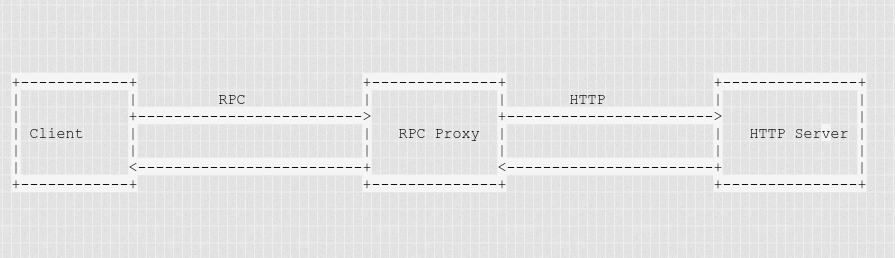
\includegraphics[scale=0.5]{RPC_topic}
\\
\\
In this project, our requirement is that the
client and the proxy will communicate through RPC protocol.
There are 2 ways to understand it:\\
\\
Firstly, the proxy can provide severial HTTP generate
function so that the client can use to send request to
the destination host (Of course the function call in here
is remote - RPC function).
But I think it is not preference way for 2 reason. It is
not productive and the general user can not used.
And the other way will be providing the data transfer proxy
as normal proxy and applying the RPC as the protocol. In
other other word, the client give proxy poorly HTTP as
data and we help them transfer it to destinate. And in
the middle of the line, the RPC protocol will be used.\\
\\
Developing from second idea, the proxy can split out or
we can say it is distributed proxy. Basicaly, there are
2 parts in the proxy system, the bunch of servers will
get the client HTTP request and the other server send request
HTTP to the destination host. The RPC is used as main protocol
between 2 type server of system.\\
\\
Why do we run this project ?\newline Obviously, this is our final
and the sub reason is the knowledge that I can gain about
proxy. And it sound very cool also.
\section{Objective}
My purpose in this project is understand the proxy definition
and use it to develope the runable proxy between the real browser
(in this case is the firefox) and any destination HTTP and HTTPS
host. During building idea time, I decide to implement 2 type server:
\begin{itemize}
\item The client proxy server which stand in the same region as
the client and can have multi-server across each geography space.
It will sit in demo computer for convenient reason. This server type
handle the client request send in as poor HTTP or HTTPS. Parse the
client request to get IP and port of destinate host, talk to other
type server (RPC protocol) to open tunnel between client and 
destination.
\item Other type server in here is the server proxy server. 
It is a bad name (I know). But it is the important part in 
my proxy system. It run outside of the censored region. Waiting
for incomming request of the client server (in RPC protocol).
Creating TCP socket to destination host, then open tunnel between
client and host website. It keep the role as end user in the
website point of view.
\end{itemize}
Note that my browser is firefox 74 so the communication with
client will follow standard of firefox 74 in proxy mode.
\section{State of the art}
Unfortunately, we could not found any the proxy server apply
RPC protocol into the commnucation. It can be explained because
most of the proxy system work as a single station. That mean
the user will send the request to a server and that server itself
sends request to the destination host. That is a simple and easy
implemented method.\\
\\
However, it is lack of security protection when the single location
of the proxy server can be found. Then the middle-man can track out
the client IP to identify the user location. But if the proxy system
are distributed as my idea, even if the part connect to the website
be found, it is still be hard to keep tracking the user IP because
the user dont connect directly to tracked server. Moreover, it is
easier to scale up sysetm. Basicaly, the server proxy part do 1 job
only is transfer data the host website. And the hard part which is
handle request from the user (include multiple of proxy communicate
protocol depending on the browser type and version) stay in the client
proxy server part. Then when the proxy implement
some new feature, instead of closing the wholw system to update,
the new client proxy part will be deployed then connect to on-running
server proxy part. I call it dynamic update
\section{Method}
\section{Evaluation}
\section{Conclusion}
\end{document}